\documentclass[a4paper,12pt]{article}

\usepackage{cmap}
\usepackage{mathtext}
\usepackage[T2A]{fontenc}
\usepackage[utf8]{inputenc}
\usepackage[english,russian]{babel}
\usepackage{listings}

\usepackage{amsmath,amsfonts,amssymb,amsthm,mathtools}
\usepackage{icomma}
\usepackage{upgreek}
\mathtoolsset{showonlyrefs=true}

\usepackage{tabto}
\usepackage{euscript}
\usepackage{mathrsfs}

\usepackage{graphicx}

\newcommand*{\hm}[1]{#1\nobreak\discretionary{}
{\hbox{$\mathsurround=0pt #1$}}{}}

\author{Kupriyanov Kirill}
\title{Data Analysis PI\\Theoretical assignment $\#4$}
\date{}

\begin{document}
\maketitle
\thispagestyle{empty}
\newpage
\section*{Task 1.}
\underline{\textit{Problem:}} The more parameters are included in machine
learning algorithm, the more it is biased to overfitting.  Indeed, overfitting
means ``flexibility'' of the model towards each observation, that in turn means
high ``degree of freedom''(large number of parameters).\\
\newline
Consider classification results of two methods: Linear
classifier (Figure 1) and K-Nearest Neighbour classifier (Figure 2). In
\(m\)-dimensional space linear classifiers have about \(m\) weight parameters,
while kNN has a single one – the number of nearest neighbours.\\
\newline
Not only from that particular case it is clear, that despite having only one
parameter, the decision boundary of kNN is more complex and flexible, as
opposite to linear classifier solution. But that contradicts the valid argument
about flexibility and the number of parameters! Why is this happening with kNN?
Justify your answer.

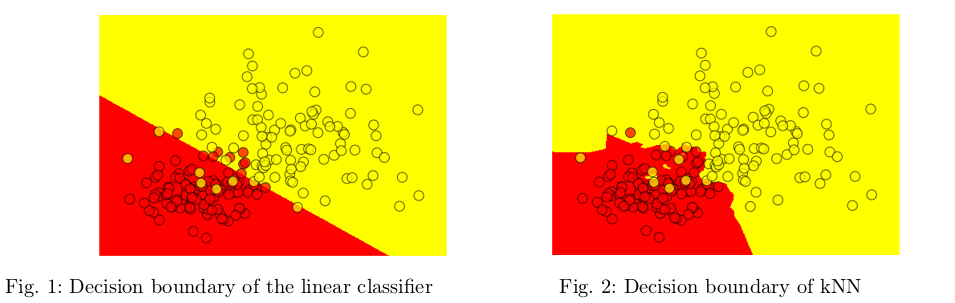
\includegraphics[width=\textwidth]{classifiers}
\newline
\underline{\textit{Solution:}} A classifier is linear if its decision boundary
on the feature space is a linear function: positive and negative examples are
separated by a \textbf{hyperplane}. By it's defenition, it cannot be
``flexible'' and non-linear. On the opposite, nonlinearity of kNN is
intuitively clear when looking at examples like Figure 2. The decision
boundaries of kNN are locally linear segments, but in general have a complex
shape that is not equivalent to a line in 2D or a hyperplane in higher
dimensions.\\
\newline
This is because KNN is non-parametric, i.e.\ it makes no assumption about the
data distribution. It just finds \(k\) closest neighbours for each sample in
the space. On the contrast, linear classifier has \(m\) parameters in the \(m\)-featured space, because the desicion hyperplane has weights \(\beta_i\); \(i\in[1,m]\).

\newpage
\section*{Task 2.}
\underline{\textit{Problem:}} A student has implemented perception algorithm for linearly separable dataset (learning rate is equal
to 1). Find a mistake in he following code listing:
\begin{lstlisting}[mathescape]
Initialize weights: $w = (w_1, \dots, w_d) = 0$
Until no errors on train set:
    i = GetRandomIndex()
    if $y_i\langle x_i, w\rangle < 0:$
        $w = w + y_ix_i$
\end{lstlisting}
\underline{\textit{Solution:}} The mistake is that all weights are initialized
with the same number, in this case, zeroes. The thing is, that during forward
propagation, every neuron gets sum of inputs, multiplied by weights. And if
weights are initialized as the same numbers (e.g., zeroes or ones), each hidden
neuron will get the same signal. This can cause symmetry in the whole
perception when backpropagating. So in this case, all units in the same layer
will be the same.

\newpage
\section*{Task 3.}
\underline{\textit{Problem:}} Consider a linearly separable dataset. Write down ML loss function for logistic regression. Show that
the maximum likelihood solution for the logistic regression model is obtained by finding a vector \(w\) and
\(w_0\) with all coefficients tend to infinity.
Name a technique that can help to overcome this issue.\\
\newline
\underline{\textit{Solution:}} The binomial likelihood function looks like
follows:

\[
    L = \sum_it_i\log(p_i) + (1-t_i)\log(1-p_i)
\]
In each term in the summation only one of \(t_i\log(p_i)\) or
\((1-t_i)\log(1-p_i)\) is non-zero, with a contribution of \(p_i\) for \(t_i =
1\) and \(1-p_i\) for \(t_i = 0\).\\
\newline
To be more accurate, the following could be written:
\[
    S(\beta,x) = \frac{1}{1+\exp(-\beta x)}
\]

for the sigmoid function. There are also two limits, each approaching limit monotonically:
\begin{align}
    \lim_{\beta\rightarrow\infty} S(\beta,x) &= 0 \text{ for  }x < 0\\
    \lim_{\beta\rightarrow\infty} S(\beta,x) &= 1 \text{ for  }x > 0
\end{align}
The first limit is decreasing, the second is increasing. Each of these follows easily from the formula for \(S\).


\end{document}


% EOF

